\chapter{Fondements théoriques et revue de la littérature sur l'IA générative et les systèmes de recommandation}
\vspace{-1.4cm}

Ce chapitre situe le mémoire dans la littérature sur l'appariement emploi-compétences, les systèmes de recommandation, les grands modèles de langage, la recherche augmentée par récupération et les graphes de connaissances. L'objectif n'est pas de reprendre mécaniquement l'histoire complète de l'intelligence artificielle ou des systèmes de recommandation. Il s'agit plutôt de sélectionner les résultats établis qui éclairent directement le problème étudié : recommander des offres, des compétences et des trajectoires de montée en qualification à partir de données hétérogènes, textuelles et relationnelles.

La revue est organisée autour d'une question directrice : pourquoi un système emploi-compétences ne peut-il pas se limiter à une recherche par mots-clés ou à un modèle génératif isolé ? La littérature montre que ce problème combine au moins quatre difficultés : les frictions du marché du travail, la variabilité du langage utilisé pour décrire les compétences, le besoin d'explicabilité dans la recommandation et le risque d'hallucination des modèles génératifs. Ces acquis justifient l'architecture retenue dans ce mémoire : embeddings sémantiques pour la proximité de contenu, graphe de connaissances pour les relations métier-compétence-formation, base vectorielle pour la recherche efficace, et orchestration agentique pour contrôler la génération finale.

\section{Marché de l'emploi, information imparfaite et appariement}

Le problème traité dans ce mémoire relève d'abord de l'économie du travail. Les modèles de recherche et d'appariement montrent que le chômage peut coexister avec des postes vacants lorsque la rencontre entre travailleurs et entreprises est coûteuse, lente ou imparfaitement informée \cite{mortensen1994job,pissarides2000equilibrium}. Cette lecture est importante : un système de recommandation emploi-compétences n'est pas seulement un outil informatique ; c'est un dispositif d'intermédiation qui cherche à réduire les coûts de recherche et à améliorer la qualité des mises en relation.

La littérature sur l'asymétrie d'information renforce ce diagnostic. Akerlof montre que l'incertitude sur la qualité peut dégrader les échanges lorsque les acteurs ne disposent pas de signaux fiables \cite{akerlof1970lemons}. Sur le marché de l'emploi, cette asymétrie apparaît des deux côtés : le recruteur ne voit pas toujours les compétences réelles du candidat, et le candidat ne connaît pas toujours les exigences effectives du poste. La théorie du signalement de Spence explique alors le rôle des diplômes, certifications et expériences comme signaux observables \cite{spence1973job}. Mais ces signaux restent incomplets lorsque les métiers évoluent rapidement, notamment dans les domaines numériques où les compétences techniques sont souvent décrites par des formulations instables.

La théorie du capital humain rappelle enfin que la formation et l'expérience sont des investissements productifs \cite{becker1964human}. Toutefois, la possession d'un capital humain ne garantit pas l'appariement. Encore faut-il que les compétences acquises soient visibles, comparables et alignées sur les compétences demandées. Autor montre que le progrès technique transforme surtout les tâches composant les métiers, et non uniquement les intitulés d'emploi \cite{autor2013growth}. Pour un système de recommandation, cela impose de descendre au niveau des compétences et des tâches plutôt que de s'arrêter aux titres de poste.

L'acquis principal de cette littérature est donc clair : le matching emploi-compétences est un problème d'information structurée. Le manque identifié est tout aussi clair : les modèles économiques expliquent les frictions, mais ils ne fournissent pas directement une architecture technique pour extraire, normaliser, comparer et expliquer les compétences dans des données textuelles. C'est précisément l'espace occupé par les méthodes de recommandation, les représentations sémantiques et les graphes de connaissances.

\section{Systèmes de recommandation : familles de méthodes et limites}

Les systèmes de recommandation cherchent à classer des items selon leur pertinence probable pour un utilisateur. La littérature distingue classiquement les approches fondées sur le contenu, le filtrage collaboratif et les approches hybrides \cite{adomavicius2005toward,ricci2011recommender}. Dans le contexte de ce mémoire, l'utilisateur peut être un candidat, un conseiller emploi ou une plateforme ; les items peuvent être des offres, compétences, métiers ou formations.

Les approches fondées sur le contenu utilisent les caractéristiques explicites des items et des profils. Elles sont adaptées au matching emploi-compétences parce que les offres et les candidats possèdent des descriptions textuelles, des secteurs, des niveaux et des compétences. Pazzani et Billsus montrent que ces systèmes exploitent les attributs des contenus pour produire des recommandations personnalisées \cite{pazzani2007content}. Leur avantage est l'interprétabilité : on peut expliquer qu'une offre est recommandée parce qu'elle partage des compétences avec le profil. Leur limite est la dépendance au vocabulaire observé. Une recherche strictement lexicale peut manquer des équivalences comme \og analyse de données \fg{}, \og data analytics \fg{} et \og reporting décisionnel \fg{}.

Le filtrage collaboratif exploite les interactions passées entre utilisateurs et items. Les approches de factorisation matricielle ont fortement structuré ce domaine en apprenant des facteurs latents à partir des matrices d'interactions \cite{koren2009matrix}. Les modèles neuronaux ont ensuite généralisé cette logique, par exemple avec le Neural Collaborative Filtering \cite{he2017ncf}. Ces méthodes sont puissantes lorsque l'on dispose d'un historique dense : clics, candidatures, recrutements, évaluations ou parcours de formation. Dans le cas du marché de l'emploi camerounais étudié ici, cette hypothèse est fragile. Les données d'interaction sont limitées, les offres changent vite et de nombreux candidats ou métiers se trouvent en situation de démarrage à froid.

Les approches hybrides combinent plusieurs sources de signal pour compenser les limites propres à chaque famille. Burke montre que l'hybridation peut améliorer la robustesse en associant contenu, collaboration, connaissances et règles métier \cite{burke2002hybrid}. Pour ce mémoire, cette conclusion est centrale : un score vectoriel peut détecter une proximité sémantique, mais il ne vérifie pas à lui seul le niveau de formation, les compétences obligatoires ou la cohérence de la trajectoire. À l'inverse, un graphe de compétences peut expliquer une relation, mais il dépend de la couverture et de la qualité des données. La bonne solution n'est donc pas de choisir entre contenu, graphe et règles ; elle consiste à organiser leur complémentarité.

\section{Recommandation emploi-compétences et spécificité du person-job fit}

La recommandation d'emploi se distingue de la recommandation de films ou de produits. Une offre n'est pas seulement un item susceptible de plaire ; elle impose des contraintes de qualification, d'expérience, de localisation, de disponibilité et de compétences. La littérature récente sur le \emph{person-job fit} insiste sur cette double sélection : le candidat doit être intéressé par l'offre, mais l'employeur doit aussi pouvoir considérer le profil comme compatible \cite{yang2022twoway}. La recommandation devient donc un problème bilatéral.

Cette spécificité change l'interprétation des scores. Dans le commerce électronique, une recommandation peut viser la probabilité de clic ou d'achat. Dans l'emploi, une recommandation doit distinguer au moins trois situations : le candidat est immédiatement compatible ; le candidat est proche mais nécessite une montée en compétences ; le candidat est trop éloigné du poste cible. La notion de \emph{skill gap} devient alors centrale. Elle consiste à comparer les compétences possédées par le candidat avec celles requises par l'offre ou le métier, puis à identifier les écarts critiques.

Les travaux récents mobilisant les graphes et les LLMs dans les ressources humaines vont dans ce sens. HRGraph propose par exemple d'exploiter des graphes de connaissances enrichis par LLM pour la recommandation d'emploi \cite{wasi2024hrgraph}. D'autres travaux s'intéressent à la prédiction des compétences et à la construction de graphes de talents pour les ressources humaines \cite{yang2025talentgraph}. Ces contributions confirment l'intérêt des graphes pour représenter les relations entre compétences, métiers et profils. Leur limite, pour notre contexte, est qu'elles ne résolvent pas automatiquement la question de l'ancrage local : nomenclatures camerounaises, données réelles de plateforme, contraintes de formation et explication opérationnelle pour un conseiller ou un candidat.

Le positionnement du mémoire se situe donc dans cet espace : adapter les acquis des systèmes de recommandation et des graphes de connaissances à un problème local d'intermédiation emploi-compétences, en intégrant des référentiels comme la \MEPC{} et la \NCF{}.

\section{IA générative et grands modèles de langage}

Les grands modèles de langage ont transformé le traitement automatique du langage naturel en permettant des tâches de génération, synthèse, reformulation et raisonnement assisté. Leur rupture technique vient principalement de l'architecture Transformer proposée par Vaswani et al., fondée sur le mécanisme d'attention \cite{vaswani2017attention}. Avant cette rupture, les représentations textuelles étaient passées des sacs de mots aux embeddings denses comme Word2Vec, qui apprennent des vecteurs capturant des régularités sémantiques et syntaxiques \cite{mikolov2013distributed}. Les mécanismes d'attention introduits en traduction neuronale ont ensuite permis aux modèles de pondérer dynamiquement les parties pertinentes d'une séquence \cite{bahdanau2015neural}.

\begin{figure}[H]
  \centering
  \caption{Évolution simplifiée des modèles de langage et des représentations textuelles}
  \label{fig:chronologie_llm_revue}
  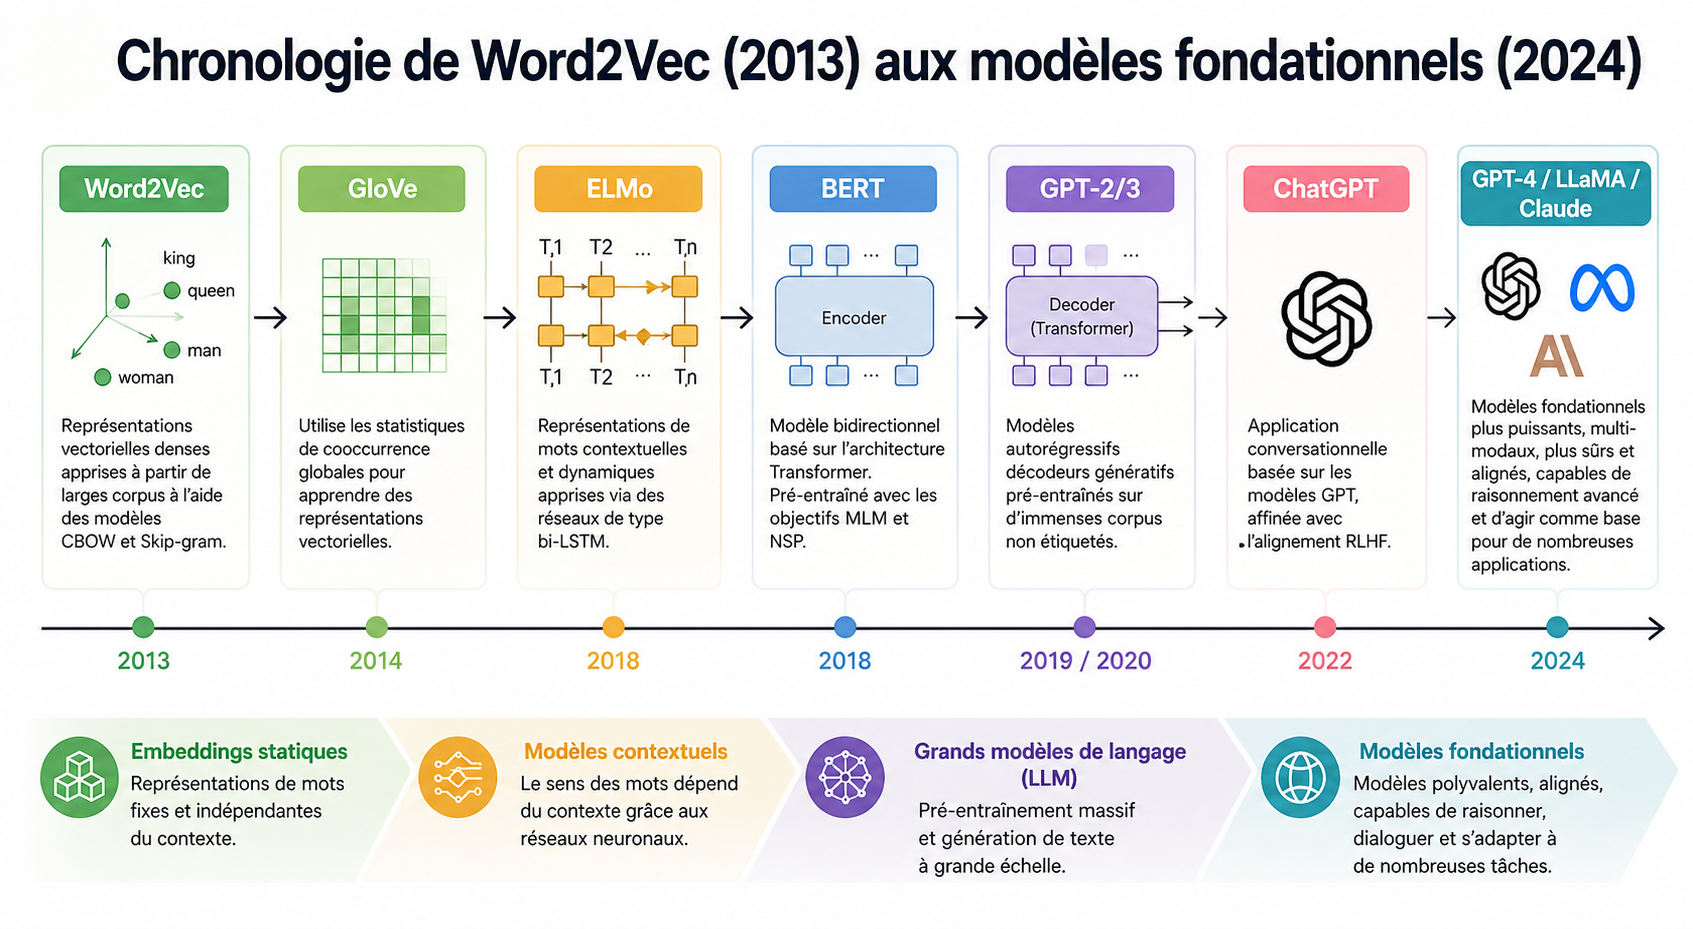
\includegraphics[width=0.75\textwidth]{figures/evolution_llms.png}
  \source{Figure du dossier du projet, synthèse pédagogique de l'évolution des modèles de langage}
\end{figure}

Deux grandes familles de modèles sont utiles pour ce mémoire. La première regroupe les modèles de représentation, comme BERT et Sentence-BERT. BERT apprend des représentations contextuelles bidirectionnelles adaptées à la compréhension du texte \cite{devlin2018bert}. Sentence-BERT adapte cette logique pour produire des embeddings de phrases comparables efficacement par similarité cosinus \cite{reimers2019sbert}. Ces modèles sont directement utiles pour rechercher des offres proches d'un profil ou des compétences proches d'une requête.

La seconde famille regroupe les modèles génératifs, comme GPT, T5 ou les modèles instruction-tuned. GPT-3 a montré qu'un modèle de grande taille pouvait effectuer des tâches variées à partir de quelques exemples dans le prompt \cite{brown2020language}. T5 a proposé une formulation unifiée des tâches NLP comme transformation texte-vers-texte \cite{raffel2020t5}. L'apprentissage par retour humain a ensuite amélioré la capacité des modèles à suivre des instructions et à produire des réponses plus alignées avec les attentes humaines \cite{ouyang2022training}.

L'acquis de cette littérature est considérable : les LLMs savent reformuler, synthétiser et produire des explications lisibles. Mais le manque est décisif pour un mémoire professionnel : un LLM ne constitue pas une base de vérité. Il peut générer une réponse plausible sans être fondée sur les données locales. Dans un système d'emploi, cette limite est critique, car une mauvaise recommandation peut orienter un candidat vers une trajectoire inadaptée. Le LLM doit donc être utilisé comme composant de génération contrôlée, et non comme moteur autonome de décision.

\section{Embeddings, recherche sémantique et bases vectorielles}

Les embeddings transforment des textes en vecteurs numériques. Cette représentation permet de mesurer la proximité de sens entre une requête, une offre, un profil candidat ou une compétence. Les benchmarks de recherche d'information montrent que les modèles d'embeddings doivent être évalués sur des tâches variées, car un bon modèle généraliste peut être insuffisant dans un domaine spécialisé \cite{thakur2021beir,muennighoff2022mteb}. Cette observation justifie l'adaptation d'un modèle SentenceTransformer au vocabulaire emploi-compétences.

La recherche sémantique résout une partie du problème de vocabulaire. Elle permet de rapprocher des textes dont les mots diffèrent mais dont le sens est proche. Dans notre cas, elle peut relier un profil mentionnant \og SQL, tableaux de bord et statistiques \fg{} à une offre de \og data analyst \fg{}. Elle reste cependant une approximation. Deux textes proches peuvent cacher une incompatibilité : niveau insuffisant, compétence obligatoire absente, localisation incompatible ou métier trop éloigné. La similarité vectorielle doit donc être traitée comme un signal de présélection, non comme une décision finale.

La littérature sur la recherche approximative de plus proches voisins montre par ailleurs que le passage à l'échelle exige des structures d'indexation efficaces. HNSW fournit un cadre robuste pour la recherche vectorielle approximative \cite{malkov2018hnsw}, tandis que FAISS a popularisé la recherche vectorielle à grande échelle \cite{johnson2019faiss}. Dans ce mémoire, l'utilisation de PostgreSQL avec pgvector répond à une logique pragmatique : conserver les embeddings dans une base relationnelle exploitable, interrogeable et intégrable au reste du pipeline \cite{pgvector2024}.

\section{Graphes de connaissances et recommandation relationnelle}

Un graphe de connaissances représente des entités et les relations qui les relient. Hogan et al. montrent que les graphes de connaissances servent à structurer des informations hétérogènes, à rendre explicites des relations sémantiques et à soutenir des tâches de recherche ou de raisonnement \cite{hogan2021knowledge}. Dans le domaine emploi-compétences, cette représentation est naturelle : un candidat possède des compétences, une offre exige des compétences, un métier appartient à une famille, une formation prépare à certains métiers, et un niveau de formation conditionne l'accès à certaines offres.

La recommandation par graphe a également connu des avancées importantes. Les graph neural networks ont fourni des outils pour propager de l'information dans des graphes \cite{kipf2017gcn,velickovic2018gat}. LightGCN a montré que, dans la recommandation collaborative, une architecture simplifiée de propagation sur graphe pouvait être très efficace \cite{he2020lightgcn}. Ces travaux établissent l'intérêt de la structure relationnelle pour la recommandation.

Cependant, le présent mémoire ne cherche pas principalement à entraîner un GNN. Le choix méthodologique est différent : utiliser un graphe de connaissances comme support d'explication, de contraintes et de calcul du skill gap. Ce choix est plus adapté au contexte disponible. Les données d'interaction ne sont pas assez riches pour justifier un modèle collaboratif profond, tandis que les relations métier-compétence-formation sont directement interprétables. Le graphe Neo4j devient donc une couche de raisonnement symbolique et relationnel autour des résultats vectoriels.

Le manque identifié dans la littérature tient au passage du modèle général au contexte local. Les travaux sur les graphes de talents et les graphes RH montrent l'intérêt des relations entre compétences et métiers, mais ils supposent souvent des référentiels bien couverts ou des plateformes disposant d'historiques importants. Le contexte camerounais impose une construction plus prudente : articuler données locales, référentiels nationaux et référentiels internationaux sans prétendre que le graphe est exhaustif.

\section{RAG, GraphRAG et contrôle de la génération}

La génération augmentée par récupération, ou \RAG{}, combine une étape de recherche d'information et une étape de génération. Lewis et al. montrent que l'accès à une mémoire externe améliore les tâches intensives en connaissances, car le modèle ne dépend plus uniquement de ses paramètres internes \cite{lewis2020rag}. Les synthèses récentes sur la \RAG{} insistent sur les mêmes enjeux : qualité de la récupération, actualisation des connaissances, évaluation de la factualité et articulation entre retriever et générateur \cite{gao2023ragllm}.

Dans une \RAG{} classique, le système récupère des documents proches d'une requête, puis les transmet au LLM. Cette architecture est utile, mais elle reste centrée sur des passages textuels. Pour le matching emploi-compétences, cela ne suffit pas. La réponse doit aussi intégrer des relations : compétences possédées, compétences requises, niveau de formation, métier cible, secteur et formation possible. Le GraphRAG étend alors la logique de récupération vers des informations structurées par graphe. Il permet de construire un contexte plus riche : non seulement des documents, mais aussi des chemins, voisins, contraintes et faits relationnels.

\begin{figure}[H]
  \centering
  \caption{Différence fonctionnelle entre \RAG{}, GraphRAG et Agentic RAG}
  \label{fig:rag_graphrag_agentic_rag_revue}
  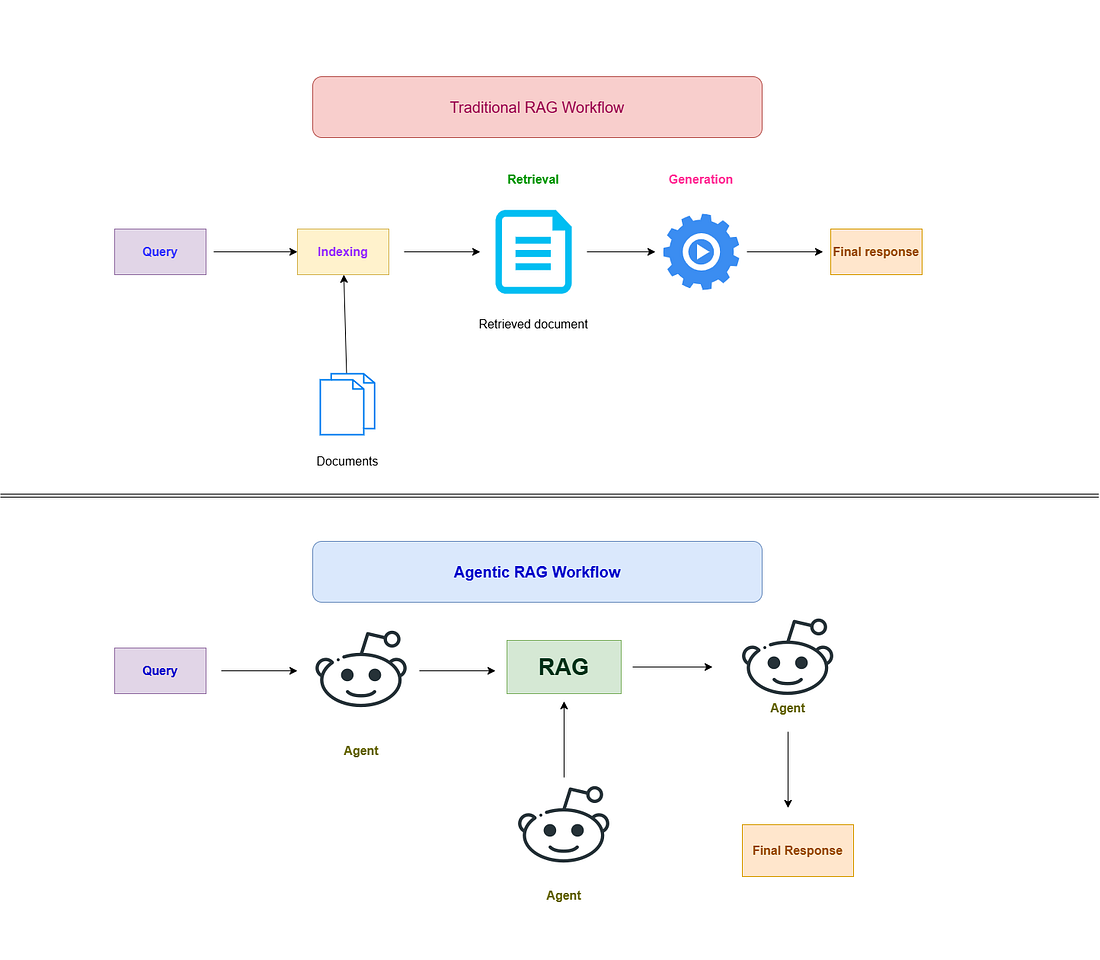
\includegraphics[width=0.92\textwidth]{figures/AgenticRAG.png}
  \source{Figure du dossier du projet, inspirée des architectures Agentic RAG et des travaux sur agents outillés}
\end{figure}

La figure \ref{fig:rag_graphrag_agentic_rag_revue} illustre cette évolution. Une \RAG{} simple suit une chaîne relativement fixe : requête, récupération, génération. Une architecture GraphRAG ajoute une couche relationnelle. Une architecture agentique introduit une capacité de planification et de contrôle : le système peut choisir un outil, observer le résultat, élargir le contexte et réviser la réponse.

Les travaux ReAct montrent l'intérêt d'alterner raisonnement et action outillée dans les modèles de langage \cite{yao2023react}. Self-RAG va plus loin en introduisant une logique d'auto-réflexion pour décider quand récupérer de l'information et comment critiquer la réponse \cite{asai2024selfrag}. Pour ce mémoire, ces travaux ne doivent pas être interprétés comme une autorisation à laisser un agent décider librement. Ils justifient plutôt une orchestration contrôlée : classifier l'intention, choisir les sources, récupérer les preuves, construire le contexte, générer, puis vérifier si la réponse est suffisamment fondée.

Le manque de la littérature est ici opérationnel. Beaucoup de travaux décrivent des architectures générales, mais la fiabilité dépend de détails concrets : qualité des chunks, schéma du graphe, robustesse des requêtes, traçabilité des sources, gestion des cas sans résultat et critères de révision. C'est pourquoi le système de ce mémoire ajoute un critic et des traces d'exécution. Le LLM produit la réponse finale, mais les données récupérées et les outils appelés doivent rester observables.

\section{Évaluation : performance, factualité et utilité professionnelle}

L'évaluation d'un système emploi-compétences ne peut pas se limiter à la fluidité de la réponse générée. La littérature en recherche d'information utilise des métriques comme Recall@k, Precision@k, MRR ou nDCG pour mesurer la capacité d'un système à retrouver des éléments pertinents \cite{thakur2021beir,muennighoff2022mteb}. Ces métriques sont nécessaires pour évaluer la recherche vectorielle et la présélection des offres.

La \RAG{} ajoute d'autres critères : fidélité au contexte, pertinence de la réponse, couverture des sources et citation des preuves. RAGAS propose par exemple un cadre d'évaluation automatisée pour des systèmes RAG \cite{es2024ragas}. G-Eval explore l'utilisation de LLMs comme juges pour l'évaluation de génération, tout en posant implicitement la question de l'alignement avec le jugement humain \cite{liu2023geval}. Ces approches sont utiles, mais elles doivent être utilisées avec prudence dans un mémoire professionnel : un juge automatique ne remplace pas une validation métier.

Dans le cas de ce projet, trois niveaux d'évaluation sont nécessaires. Le premier est technique : le système retrouve-t-il les offres, compétences ou documents pertinents ? Le deuxième est relationnel : l'ajout du graphe améliore-t-il la prise en compte des compétences et du niveau de formation ? Le troisième est professionnel : la recommandation est-elle explicable, actionnable et utile pour réduire un écart de compétences ? Cette grille justifie l'évaluation comparative entre pgvector seul et pgvector enrichi par Neo4j présentée dans le chapitre d'évaluation.

\section{Synthèse critique et positionnement du mémoire}

La littérature fournit plusieurs acquis solides. Les modèles d'appariement du marché du travail expliquent pourquoi les frictions informationnelles justifient des dispositifs d'intermédiation. Les systèmes de recommandation montrent que l'hybridation est souvent nécessaire lorsque les données sont hétérogènes. Les Transformers et les embeddings permettent de dépasser la recherche lexicale. Les graphes de connaissances apportent une structure relationnelle utile pour expliquer les recommandations. La \RAG{} et l'Agentic RAG permettent enfin de produire des réponses en langage naturel à partir de contextes récupérés.

Mais ces acquis laissent des manques importants. Premièrement, une proximité sémantique n'est pas une preuve de compatibilité professionnelle. Deuxièmement, les modèles collaboratifs exigent des historiques d'interaction souvent absents dans les plateformes émergentes. Troisièmement, un LLM peut formuler une réponse convaincante sans être fidèle aux données. Quatrièmement, les graphes RH proposés dans la littérature ne sont pas automatiquement adaptés aux nomenclatures camerounaises ni aux données locales de KmerAI.

Le domaine de recherche du mémoire se situe donc à l'intersection de la recommandation hybride, des graphes de connaissances et de la génération contrôlée. La contribution n'est pas de proposer un nouveau Transformer ou un nouvel algorithme de factorisation matricielle. Elle consiste à concevoir et évaluer une architecture intégrée pour le matching emploi-compétences : recherche sémantique par embeddings, stockage vectoriel avec pgvector, structuration relationnelle avec Neo4j, interrogation GraphRAG, critic de réponse et génération finale avec un \LLM{} contraint par le contexte.

Cette position est volontairement prudente. Le système ne prétend pas remplacer l'expertise humaine du conseiller emploi ou du recruteur. Il vise à rendre l'information plus exploitable : quelles offres sont proches du profil, quelles compétences expliquent la recommandation, quels écarts subsistent, et quelles pistes de formation peuvent réduire ces écarts. C'est cette articulation entre performance algorithmique, explicabilité et utilité professionnelle qui guide les choix méthodologiques et l'implémentation présentés dans les chapitres suivants.
